\subsection{Caso particular: Entrevistas}

  \paragraph{}Como se puede observar en la figura \ref{diagramaEntrevista}, las
  entidades \textit{Entrevista}, \textit{Entrevista General} y
  \textit{Entrevista Asesor} forman una relación jerárquica que es
  conveniente eliminar para poder utilizar mecanismos útiles para transformar el
  esquema conceptual a relacional.

  \paragraph{}Teniendo en cuenta la naturaleza de la relación jerárquica, cuya
  especialización es de dos subtipos de entidad con respecto al tipo de entidad
  general, y cuyo tipo de especialización es total y sin solapamiento, se ha
  utilizado la regla PRTECAR-3\footnote{Regla PRTECAR-3: \textit{Eliminación del
  supertipo de entidad: En un tipo de interrelación jerárquica se desestimará el
  supertipo de entidad, transfiriendo todos los atributos del supertipo a cada
  uno de los subtipos y cada uno de los tipos de interrelación que mantuviera el
  supertipo de entidad serán considerados para cada uno de los subtipos,
  manteniéndose, por supuesto, los tipos de interrelación en los que intervengan
  cada uno de los subtipos de entidad. Además, el atributo cualificador del tipo
  de interrelación, si estuviera presente, se puede desestimar. Si el tipo de
  interrelación jerárquica es exclusivo, los subtipos intervendrán de forma
  parcial (cardinalidad mínima cero) en los tipos de interrelación transferidos
  desde el supertipo.}}.

  \paragraph{}Tras aplicar dicha regla, el supertipo de entidad
  \textit{Entrevista} desaparece, dando como resultado la figura
  \ref{diagramaEntPreg}. Aplicando las distintas reglas para transformar los
  esquemas conceptuales a relacionales se obtienen las siguientes tablas:

  \begin{itemize}
    \item Tabla EntrevistasGenerales.
    \item Tabla EntrevistasAsesores.
    \item Tabla Preguntas.
    \item Tabla EntrevistaGeneral\_Asesores.
  \end{itemize}

  \begin{figure}[!ht]
    \begin{center}
      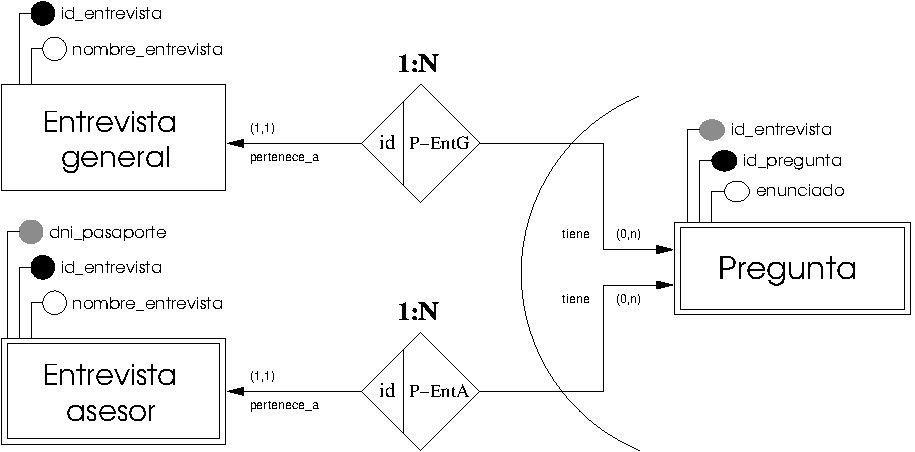
\includegraphics[]{10.Disenyo_Datos/10.2.Modelo_Datos_Relacional/Tablas/diagramas/Entrevistas-Pregunta.pdf}
      \caption{Diagrama Entrevistas\_Preguntas.}
      \label{diagramaEntPreg}
    \end{center}
  \end{figure}